\documentclass{report}

% Packages nécessaires
\usepackage[utf8]{inputenc}
\usepackage[T1]{fontenc}
\usepackage[french]{babel}
\usepackage{titlesec}
\usepackage{tocloft}
\usepackage{lipsum} % Package de remplissage de texte (à retirer dans le rapport final)
\usepackage{graphicx}
\usepackage{float} % pour l'option de placement [H]
\usepackage[colorlinks=true, linkcolor=blue, citecolor=green]{hyperref}
\usepackage{minted} % pour la coloration syntaxique
\usepackage{lipsum}
\usepackage{wrapfig}   % Pour l'enroulement du texte autour des images
\usepackage{array}

% Mathématiques
\usepackage{amsmath, amssymb}
\usepackage{amsthm}
\usepackage{mdframed}  % Package pour les cadres

% Environnements pour les théorèmes, définitions et preuves
\newtheorem{theorem}{Théorème}
\newtheorem{definition}{Définition}
\newtheorem{example}{Exemple}
\newtheorem{property}{Propriété}

\newmdtheoremenv{boxedproperty}{Propriété}[section]  % Crée un environnement encadré pour les propriétés


% Configuration de la page
\usepackage[a4paper, left=2.5cm, right=2.5cm, top=2.5cm, bottom=2.5cm]{geometry}

% Pour avoir le petit dessin de l'INSA en bas à droite de chaque page
\usepackage{background}
\backgroundsetup{
scale=1,
angle=0,
opacity=1,
color=black,
contents={\begin{tikzpicture}[remember picture,overlay]
\node at ([xshift=-0.8in,yshift=0.8in] current page.south east) % Adjust the position of the logo.
{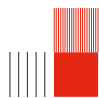
\includegraphics[scale=0.8]{images/pattern.png}}; % logo goes here
\end{tikzpicture}}
}


% Configuration des titres des sections et sous-sections
\titleformat{\chapter}[display]
  {\normalfont\huge\bfseries}{\chaptertitlename\ \thechapter}{20pt}{\Huge}
\titleformat{\section}
  {\normalfont\Large\bfseries}{\thesection}{1em}{}
\titleformat{\subsection}
  {\normalfont\large\bfseries}{\thesubsection}{1em}{}

% Configuration de la table des matières
\renewcommand{\cftchapfont}{\bfseries}
\renewcommand{\cftsecfont}{\normalfont}
\renewcommand{\cftsubsecfont}{\normalfont}
\renewcommand{\cftchappagefont}{\bfseries}
\renewcommand{\cftsecpagefont}{\normalfont}
\renewcommand{\cftsubsecpagefont}{\normalfont}
\setlength{\cftbeforetoctitleskip}{0pt}
\setlength{\cftaftertoctitleskip}{10pt}
\renewcommand{\contentsname}{Table des matières}



\begin{document}


% --- PAGE DE TITRE ---
\begin{titlepage}
    \centering
    \noindent 
    \begin{minipage}{0.45\textwidth}
        
\includegraphics[width=0.8\linewidth]{images/logo_INSA.png} 
    \end{minipage}%
    \hfill 
    \begin{minipage}{0.45\textwidth}
        \flushright 
        
\includegraphics[width=0.8\linewidth]{images/tescan_logo.png} 
    \end{minipage}

    \vspace*{2cm} 
    {\Huge\bfseries Rapport de Projet Multidisciplinaire \par}
    \vspace{1cm}
    {\huge Modélisation du Quadrupôle d'Okayama par BEM \par}
    \vspace{0.4cm}
    {\large (\textit{Boundary Element Method}) \par}
    \vspace{2cm}

    {\Large \textbf{Zoé \textsc{Nonon} --- Louise \textsc{Lammertyn}} \par}
    \vspace{0.2cm}
    {\large $4^{\text{ème}}$ année Génie Physique \par}
    
    \vspace{2.5cm}

    {\large \textbf{Tuteurs :}} \par
    \vspace{0.5cm}
    {\large
    \begin{tabular}{l}
        Florent \textsc{Houdellier} \\
        Lucile \textsc{Berdoux Durieux} \\
        Jean-Baptiste \textsc{Mellier} \\
        Pier-Francesco \textsc{Fazzini}
    \end{tabular}
    } \par
    
    \vfill 
    {\large Année universitaire 2025-2026 \par}
    \vspace{0.8cm}
    {\Large \textbf{Institut National des Sciences Appliquées de Toulouse} \par}
    \vspace{0.5cm}
    {\large \today \par}
\end{titlepage}

% Résumé concis, souvent utilisé pour donner un aperçu rapide du contenu d'une recherche ou d'un article académique.
\begin{abstract}
    balblabalba % Lorem Ipsum
\end{abstract}

% Table des matières
\tableofcontents

% Début du contenu du rapport
\chapter{Introduction}

\label{sec:cats}

Les chats (\emph{Felis catus}) sont parmi les animaux domestiques les plus populaires au monde. Voici pourquoi ils sont tant appréciés :

\begin{itemize}
    \item \textbf{Indépendance} : Les chats sont réputés pour leur nature indépendante.
    \item \textbf{Comportement affectueux} : Ils peuvent être très affectueux et sociaux avec leurs propriétaires.
    \item \textbf{Facilité de soins} : Ils nécessitent moins de soins quotidiens que les chiens.
\end{itemize}


\par % Nouveau paragraphe
\smallskip % Petit espace entre les paragraphes
\noindent % Pas d'indentation
Les chats ont aussi une grande variété de \textbf{\emph{comportements}} qui fascinent leurs observateurs. Par exemple, le ronronnement, souvent associé à un état de bien-être, reste un mystère pour les scientifiques. Pour plus d'informations, voir la section \ref{sec:behaviors} sur les comportements spécifiques.

\section{Contexte}
\label{sec:behaviors}
\noindent % Pas d'indentation
Les chats ont des comportements qui sont à la fois intrigants et diversifiés. Leur capacité à sauter de grandes hauteurs ou leur agilité remarquable sont des traits bien connus. Pour en savoir plus, consultez \href{https://fr.wikipedia.org/wiki/Chat}{wikipedia} pour des détails et des anecdotes sur ces fascinantes créatures.


\chapter{Contenu du rapport}

\section{Les chat-soupis}


\lipsum[100]

\par % Nouveau paragraphe
\bigskip % Grand espace entre les paragraphes
\noindent % Pas d'indentation pour le paragraphe suivant
Exemples citations liées à la bibliographie : Dans cette section, nous discutons de travaux antérieurs. Comme indiqué par \cite{smith2023}, \cite{johnson2024}, et \cite{doe2025}... La méthodologie employée est largement inspirée par celle décrite par \cite{johnson2024}. Pour plus de détails, veuillez consulter les travaux de \cite{doe2025}.

\newpage % Nouvelle page

\section{Les chats mignons}

Les chats sont souvent perçus comme étant particulièrement mignons pour plusieurs raisons. Premièrement, leurs traits physiques, tels que leurs grands yeux ronds, leurs petites oreilles pointues, et leur fourrure douce, évoquent un sentiment de douceur et de fragilité qui stimule notre instinct de protection. Ce phénomène, connu sous le nom de "réponse de mignoncité," est une réaction émotionnelle qui nous pousse à prendre soin de créatures qui semblent vulnérables ou enfantines.
\par % Nouveau paragraphe
\smallskip % Petit espace entre les paragraphes
\noindent % Pas d'indentation
Ensuite, le comportement des chats contribue également à leur charme. Leur penchant pour les jeux et leurs mouvements agiles leur donnent un air jovial et divertissant. De plus, les chats ont une façon unique de montrer leur affection, que ce soit par des ronronnements apaisants ou des petits coups de tête affectueux, ce qui renforce le lien émotionnel entre l'animal et son propriétaire.
\par % Nouveau paragraphe
\smallskip % Petit espace entre les paragraphes
\noindent
Enfin, les chats possèdent une indépendance qui les rend intrigants et parfois même comiques dans leurs interactions avec les humains. Cette combinaison de dépendance affective et d'autonomie crée une dynamique fascinante qui captive souvent les amoureux des animaux.
\par % Nouveau paragraphe
\smallskip % Petit espace entre les paragraphes
\noindent
En somme, l'attrait des chats repose sur un mélange complexe de traits physiques attrayants, de comportements engageants, et d'une personnalité à la fois indépendante et affectueuse, ce qui les rend irrésistiblement mignons à nos yeux.
\par % Nouveau paragraphe
\medskip % Moyen espace entre les paragraphes
\noindent
Au-delà de leur apparence et de leur comportement, les chats communiquent aussi de manière très efficace grâce à leurs expressions faciales et à leur langage corporel. Par exemple, le simple fait qu’un chat cligne lentement des yeux en votre présence peut être interprété comme un signe de confiance et d'affection, un geste qui est souvent appelé "le baiser de chat". Ces subtilités de communication renforcent la perception de leur mignonnerie car elles créent une connexion émotionnelle profonde entre le chat et son humain.
\par % Nouveau paragraphe
\smallskip % Petit espace entre les paragraphes
\noindent
La science elle-même s'est penchée sur la question de la mignonnerie des chats. Des études ont montré que regarder des vidéos de chats peut réduire le stress et augmenter les sentiments de bonheur chez les humains. Cette réponse émotionnelle positive est une autre raison pour laquelle les gens trouvent les chats si adorables. Ils ne sont pas seulement mignons à regarder, mais leur présence peut avoir un impact bénéfique réel sur notre bien-être émotionnel.

\newpage % Nouvelle page

\section{Les chat-pardeurs}

Les chats chapardeurs, souvent décrits comme des petits voleurs félins, ajoutent une dimension à la fois amusante et frustrante à la vie de leurs propriétaires. Ces comportements, bien que parfois source de tracas, peuvent en fait être révélateurs de plusieurs aspects de la psychologie féline et de l'environnement domestique dans lequel les chats évoluent.
\par % Nouveau paragraphe
\smallskip % Petit espace entre les paragraphes
\noindent % Pas d'indentation
Pour commencer, il est important de comprendre que les chats sont par nature des prédateurs. Leurs instincts de chasseur les poussent à pourchasser tout ce qui bouge, ce qui inclut parfois des objets qui ne sont pas destinés à être des jouets. Ainsi, un chat peut être attiré par un objet brillant ou mobile, le percevant comme une proie potentielle. Cela explique pourquoi de nombreux chats sont attirés par des objets tels que des stylos, des bijoux ou même des petits appareils électroniques. Ces objets, lorsqu'ils sont emportés dans leur cachette, deviennent des trophées pour ces chasseurs miniatures.
\par % Nouveau paragraphe
\smallskip % Petit espace entre les paragraphes
\noindent % Pas d'indentation
Au-delà de l'instinct de prédation, il y a aussi un aspect de jeu dans le comportement de chapardage des chats. Les chats, surtout lorsqu'ils sont jeunes et actifs, ont besoin de stimulation constante. Chaparder des objets peut être une façon pour eux de s'engager dans un jeu auto-dirigé, surtout si la réaction de leur propriétaire à ces actes de vol est de les poursuivre ou de chercher l'objet perdu. Cela peut transformer une simple activité en une forme de jeu interactif, renforçant ainsi le comportement.


La personnalité du chat joue également un rôle clé dans son penchant pour le chapardage. Certains chats sont naturellement plus curieux et aventureux que d'autres, ce qui peut les inciter à explorer des zones qui ne leur sont normalement pas accessibles, comme des tiroirs ou des sacs à main laissés ouverts. Une fois qu'ils découvrent que ces endroits contiennent des objets intéressants à jouer ou à transporter, ils peuvent développer une habitude de fouiller ces espaces régulièrement.

\chapter{Mathématiques}

\section{Algèbre Linéaire}
\subsection{Vecteurs et espaces vectoriels}
\begin{definition}
Un \textbf{espace vectoriel} sur un corps \(\mathbb{F}\) est un ensemble \(V\) accompagné de deux opérations : addition vectorielle et multiplication scalaire, qui suivent dix axiomes, incluant la commutativité, l'associativité, et la distributivité.
\end{definition}

\begin{example}
Considérons l'espace des vecteurs \(\mathbb{R}^2\), où chaque vecteur représente une possible position d'un chat dans un plan. L'addition de deux vecteurs est analogue à calculer une nouvelle position basée sur deux déplacements successifs.
\end{example}

\begin{boxedproperty}
Si un chat marche d'un point \( A \) à un point \( B \) puis de \( B \) à un point \( C \), la vectorisation de son trajet peut être décrite par l'équation vectorielle \(\vec{AB} + \vec{BC} = \vec{AC}\). Ceci illustre la règle du parallélogramme pour l'addition de vecteurs.
\end{boxedproperty}

\section{Analyse}
\subsection{Calcul différentiel}
\begin{theorem}
Soit \(f : \mathbb{R} \to \mathbb{R}\) une fonction différentiable. Alors, la dérivée de \(f\), notée \(f'\), en tout point \(a \in \mathbb{R}\), est donnée par la limite:
\[
f'(a) = \lim_{h \to 0} \frac{f(a+h) - f(a)}{h}
\]
\end{theorem}

\begin{example}
Si un chat accélère à une vitesse variable, la fonction représentant sa position est différentiable, et sa vitesse instantanée en tout point est donnée par la dérivée de cette fonction.
\end{example}

\section{Topologie}
\subsection{Continuité}
\begin{definition}
Une fonction \(f : X \to Y\) entre deux espaces topologiques est dite \textbf{continue} si, pour tout ouvert \(V\) de \(Y\), la pré-image \(f^{-1}(V)\) est un ouvert de \(X\).
\end{definition}

\begin{example}
La continuité peut être vue comme un chat qui peut se déplacer d'un point à un autre sans sauter ni disparaître soudainement — chaque point du trajet est accessible de manière continue à partir du précédent.
\end{example}



\bibliographystyle{plain}
\bibliography{references}


\end{document}
